% Options for packages loaded elsewhere
\PassOptionsToPackage{unicode}{hyperref}
\PassOptionsToPackage{hyphens}{url}
%
\documentclass[
  ignorenonframetext,
]{beamer}
\usepackage{pgfpages}
\setbeamertemplate{caption}[numbered]
\setbeamertemplate{caption label separator}{: }
\setbeamercolor{caption name}{fg=normal text.fg}
\beamertemplatenavigationsymbolsempty
% Prevent slide breaks in the middle of a paragraph
\widowpenalties 1 10000
\raggedbottom
\setbeamertemplate{part page}{
  \centering
  \begin{beamercolorbox}[sep=16pt,center]{part title}
    \usebeamerfont{part title}\insertpart\par
  \end{beamercolorbox}
}
\setbeamertemplate{section page}{
  \centering
  \begin{beamercolorbox}[sep=12pt,center]{part title}
    \usebeamerfont{section title}\insertsection\par
  \end{beamercolorbox}
}
\setbeamertemplate{subsection page}{
  \centering
  \begin{beamercolorbox}[sep=8pt,center]{part title}
    \usebeamerfont{subsection title}\insertsubsection\par
  \end{beamercolorbox}
}
\AtBeginPart{
  \frame{\partpage}
}
\AtBeginSection{
  \ifbibliography
  \else
    \frame{\sectionpage}
  \fi
}
\AtBeginSubsection{
  \frame{\subsectionpage}
}
\usepackage{amsmath,amssymb}
\usepackage{lmodern}
\usepackage{iftex}
\ifPDFTeX
  \usepackage[T1]{fontenc}
  \usepackage[utf8]{inputenc}
  \usepackage{textcomp} % provide euro and other symbols
\else % if luatex or xetex
  \usepackage{unicode-math}
  \defaultfontfeatures{Scale=MatchLowercase}
  \defaultfontfeatures[\rmfamily]{Ligatures=TeX,Scale=1}
\fi
% Use upquote if available, for straight quotes in verbatim environments
\IfFileExists{upquote.sty}{\usepackage{upquote}}{}
\IfFileExists{microtype.sty}{% use microtype if available
  \usepackage[]{microtype}
  \UseMicrotypeSet[protrusion]{basicmath} % disable protrusion for tt fonts
}{}
\makeatletter
\@ifundefined{KOMAClassName}{% if non-KOMA class
  \IfFileExists{parskip.sty}{%
    \usepackage{parskip}
  }{% else
    \setlength{\parindent}{0pt}
    \setlength{\parskip}{6pt plus 2pt minus 1pt}}
}{% if KOMA class
  \KOMAoptions{parskip=half}}
\makeatother
\usepackage{xcolor}
\newif\ifbibliography
\usepackage{longtable,booktabs,array}
\usepackage{calc} % for calculating minipage widths
\usepackage{caption}
% Make caption package work with longtable
\makeatletter
\def\fnum@table{\tablename~\thetable}
\makeatother
\usepackage{graphicx}
\makeatletter
\def\maxwidth{\ifdim\Gin@nat@width>\linewidth\linewidth\else\Gin@nat@width\fi}
\def\maxheight{\ifdim\Gin@nat@height>\textheight\textheight\else\Gin@nat@height\fi}
\makeatother
% Scale images if necessary, so that they will not overflow the page
% margins by default, and it is still possible to overwrite the defaults
% using explicit options in \includegraphics[width, height, ...]{}
\setkeys{Gin}{width=\maxwidth,height=\maxheight,keepaspectratio}
% Set default figure placement to htbp
\makeatletter
\def\fps@figure{htbp}
\makeatother
\setlength{\emergencystretch}{3em} % prevent overfull lines
\providecommand{\tightlist}{%
  \setlength{\itemsep}{0pt}\setlength{\parskip}{0pt}}
\setcounter{secnumdepth}{-\maxdimen} % remove section numbering
\usetheme[numbering=fraction]{metropolis}
\definecolor{beaublue}{rgb}{0.74, 0.83, 0.9}
\setbeamertemplate{frame footer}{\tiny{\textcolor{beaublue}{Workshop - Data Wrangling of Web Data in R | SIMON RESS}}}
\makeatletter
\def\ps@titlepage{%
  \setbeamertemplate{footline}{}
}
\addtobeamertemplate{title page}{\thispagestyle{titlepage}}{}
\makeatother

\makeatletter
\renewcommand{\metropolis@enablesectionpage}{
  \AtBeginSection{
    \ifbeamer@inframe
      \sectionpage
    \else
      \frame[c]{\sectionpage}
    \fi
  }
}
\metropolis@enablesectionpage
\makeatother

\makeatletter
\def\ps@sectionpage{%
  \setbeamertemplate{frame footer}{\tiny{\textcolor{beaublue}{Workshop - Data Wrangling of Web Data in R | SIMON RESS}}}
}
\addtobeamertemplate{section page}{\thispagestyle{sectionpage}}{}
\makeatother

\setbeamertemplate{section in toc}{
\leavevmode%
\inserttocsectionnumber. 
\inserttocsection\par%
}
\setbeamertemplate{subsection in toc}{
\leavevmode\leftskip=2.5em\inserttocsubsection\par}

\definecolor{shadecolor}{RGB}{240,240,240}
\let\verbatim\undefined
\let\verbatimend\undefined
\DefineVerbatimEnvironment{verbatim}{Verbatim}{frame=single, rulecolor=\color{shadecolor}, framerule=0.3mm,framesep=1mm}

\usepackage{fvextra}
\DefineVerbatimEnvironment{Highlighting}{Verbatim}{breaklines,commandchars=\\\{\}}

\ifLuaTeX
  \usepackage{selnolig}  % disable illegal ligatures
\fi
\IfFileExists{bookmark.sty}{\usepackage{bookmark}}{\usepackage{hyperref}}
\IfFileExists{xurl.sty}{\usepackage{xurl}}{} % add URL line breaks if available
\urlstyle{same} % disable monospaced font for URLs
\hypersetup{
  pdfauthor={Simon Ress \textbar{} MT AG},
  hidelinks,
  pdfcreator={LaTeX via pandoc}}

\title{\includegraphics[width=2.5in,height=\textheight]{Slides_files/RUB.jpg}}
\subtitle{Workshop: Modern Causal Analysis. Rubin Causal Model and
Directed Acyclic Graphs}
\author{Simon Ress \textbar{} MT AG}
\date{month day, 2023}

\begin{document}
\frame{\titlepage}

\begin{frame}{Content}
\protect\hypertarget{content}{}
\tableofcontents[]
\end{frame}

\hypertarget{i.-causal-hypotheses}{%
\section{I. Causal Hypotheses}\label{i.-causal-hypotheses}}

\begin{frame}{I. Causal Hypotheses}
\end{frame}

\begin{frame}{``Simple'' causal hypotheses}
\protect\hypertarget{simple-causal-hypotheses}{}
``Simple'' causal hypotheses with two feature:

\begin{itemize}
\tightlist
\item
  Graphic representation of a ``simple'' hypothesis: causal effect of a
  feature D on a feature Y
\end{itemize}

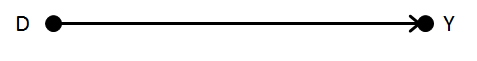
\includegraphics{Graphics/D_on_Y.png}

\begin{longtable}[]{@{}ll@{}}
\toprule()
\textbf{D} & \textbf{Y} \\
\midrule()
\endhead
Treatment variable & Outcome variable \\
Explanatory variable & Explained variable \\
Independent variable & Dependent variable \\
\bottomrule()
\end{longtable}
\end{frame}

\begin{frame}{Criteria for causal inference (D on Y)}
\protect\hypertarget{criteria-for-causal-inference-d-on-y}{}
\begin{enumerate}
\tightlist
\item
  Distinct theoretical constructs: No definitional dependency between D
  and Y
\item
  Appropriate operationalizations and measurement of both features:
  features → variables
\item
  Theoretical plausibility: Qualitative explanation (→ mechanism) of the
  causal effect necessary; reference to empirical studies not
  sufficient!
\item
  Appropriate temporal order: Theoretical justification needed
  (empirical order not sufficient, since anticipation effects can occur)
\item
  Appropriate temporal distance: Some effects take time to unfold and
  some effects weaken over time (theoretical justification needed)
\item
  Identification of the causal effect: E.g. by DAG
\item
  Empirical association: E.g. by regression analysis
\end{enumerate}
\end{frame}

\hypertarget{ii.-the-counterfactual-causal-model}{%
\section{II. The counterfactual causal
model}\label{ii.-the-counterfactual-causal-model}}

\begin{frame}{II. The counterfactual causal model}
\end{frame}

\begin{frame}{History and basic idea}
\protect\hypertarget{history-and-basic-idea}{}
\textbf{History}

▸ First approaches: John Stuart Mill 1843 \& Gustav Theodor Fechner
1860)

▸ Formal concepts of experimental designs in statistics: Neyman 1923 \&
Fisher 1935

▸ Formalized causal analysis: Donald B. Rubin 1974, 1977 \& 1978

\textbf{Basic idea}

▸ Focus on the causality concept ``Estimating the causal effect of D on
Y''

▸ Based on experimental language: almost any situation can be described
in non-experimental context at least as a thought experiment

\textbf{Other names:}

▸ Potential Outcome Model (POM)

▸ Rubin Causal Model (RCM)

▸ Modern Causal Analysis (MCA)
\end{frame}

\begin{frame}{Definitions of treatment and outcomes}
\protect\hypertarget{definitions-of-treatment-and-outcomes}{}
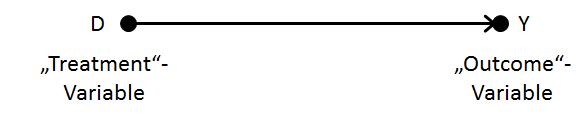
\includegraphics{Graphics/D_on_Y_names.png}

\textbf{Simplified version of a binary ``Treatment'':}

▸ D=1: Treatment (``Experimental group'')

▸ D=0: No Treatment (``Control group'')

Note: \emph{The binary treatment assumption is a simplistic assumption;
There are counterfactual causal models with polytomic treatments
(nominal, ordinal, metric).}
\end{frame}

\begin{frame}{Central assumption for outcome Y}
\protect\hypertarget{central-assumption-for-outcome-y}{}
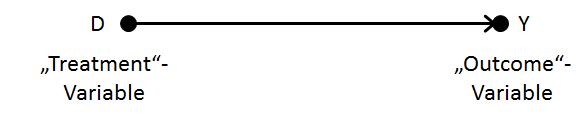
\includegraphics{Graphics/D_on_Y_names.png}

Each individual \textbf{i} can be observed in two potential states
(depending on a potential treatment), which means that \textbf{two
potential outcomes} are conceivable for each person i, regardless of the
actual treatment status: ▸
Y\textless sub\textgreater i\textless/sub\textgreater\textless sup\textgreater0\textless/sup\textgreater=
potential outcome for person i in the case without the treatment ▸
Y\textless sub\textgreater i\textless/sub\textgreater\textless sup\textgreater1\textless/sup\textgreater=
potential outcome for person i in the case of the treatment Note:
\emph{The outcome is generally viewed as metric, but other scale levels
can also be assumed.}
\end{frame}

\hypertarget{iii.-the-naive-estimator}{%
\section{III. The naive estimator}\label{iii.-the-naive-estimator}}

\begin{frame}{III. The naive estimator}
\end{frame}

\hypertarget{iv.-directed-acyclic-graphs-dags}{%
\section{IV. Directed Acyclic Graphs
(DAGs)}\label{iv.-directed-acyclic-graphs-dags}}

\begin{frame}{IV. Directed Acyclic Graphs (DAGs)}
\end{frame}

\hypertarget{v.-experimental-vs.-non-experimental-designs}{%
\section{V. Experimental vs.~non-experimental
designs}\label{v.-experimental-vs.-non-experimental-designs}}

\begin{frame}{V. Experimental vs.~non-experimental designs}
\end{frame}

\begin{frame}{End of the Preview}
\protect\hypertarget{end-of-the-preview}{}
\end{frame}

\begin{frame}{Literature}
\protect\hypertarget{literature}{}
\end{frame}

\end{document}
